\documentclass[12 pt]{article}
\usepackage[margin = 1.0in, letterpaper]{geometry}
\usepackage{graphicx}
\usepackage{amsfonts, amsmath}
\usepackage{float}

\begin{document}

\title{Interferometry and the Search For More Sources}
\author{Eduardo Herrera}

\maketitle

\begin{abstract}
For this lab, we focused on using interferometers to track
various sources across the sky from horizon to horizon using a tracking
code that followed the source for the amount of time it was visible to
the telescopes. From there data was manipulated from
these sources, starting with the point source data from the Crab Nebula (3C144).
We were able to derive values for the Declination and the Baseline (with
different codes for each to make appropriate guesses for either the
Declination or the Baseline) which
were very close to their actual values to within one percent. With the Sun
data taken for most of the day (a full observation was rendered short
by other groups' scripts not finishing) we were able to get a value
for $\phi$ and a create a wave that traced the envelope of the Sun
data. As for the Moon, there was a similar process wielding relatively
unstaisfactory results with
the same method.  
\end{abstract}


\section*{Introduction}
In the study of sources in the sky it is important to understand what
the components of the interferometer do, or be able to tell how one's
data has been affected by the telescope and equipment and be able to
correct for these affects so that as much data as possible comes from
the source itself rather than having data give results that do not
reflect past observations; in other words, noise from other sources. 
\section*{Theory and Methods}
\subsection*{Interferometry}
The most vital part for our observations, interferometry involves using
a two radio telescope array (there could be more in large arrays). The
telescopes themselves are not the interferometer, but this array along
with the electronics are. The two telescopes are separated by a baseline
vector, \textbf{b}. With a source in the direction $\hat{s}$. Plane
waves from the sources will go to one of the telescopes first with a
short delay before the same plane wave reaches the second telescope, this
delay is called the \textit{geometric delay}, $\tau$, defined by 
\begin{equation}
  \tau = \frac{\textbf{b}\hat{s}}{c}
\end{equation}
If there was another source,  then it would cause another geometric
delay and would be different from the delay of the first source and
would also have
a different $\hat{s}$. To differentiate from the sources they would need
to correlate, which is what the correlator does to differentiate between the
signals by plotting on a power spectrum, uncorrelated parts will average
out to zero when correlated and the correlated data will appear as
spikes for the signal from which
it can be determined what their $\tau$'s are by looking at the time-axis.

\subsection*{The Rotation Matrices}
Before making any measurements, a script has to be developed that takes
into account our position on earth as well as the positions of the
sources in the sky, especially the Sun and Moon, which have constantly
changing positions in the sky as opposed to the relatively still point
sources. \par
To start, most would start with longitude and latitude coordinates in
degrees but to ultimately get to  galactic coordinates (or any other
type of coordinate system) via matrices that
translate coordinates from one convention to another. If the
longitude and latitude coordinates given were in degrees rather than
radians this
procedure takes the longitude, latitude and results in right ascension,
and declination. So to
start in this example we'd have to convert from degrees to radians using the code: \par
\begin{center}
x = np.array([0.,0,0]) \par
x[0] = np.cos(np.deg2rad(lat)) * np.cos(np.deg2rad(lon)) \par
x[1] = np.cos(np.deg2rad(lat)) * np.sin(np.deg2rad(lon)) \par
x[2] = np.sin(np.deg2rad(lat)) \par
return x \par
\end{center}
after setting up this first array, to change from one coordinate system
to another requires multiplying that array by a matrix resulting in
another array that gives the new coordinates. 
\begin{equation}
  \vec{x}' = R*\vec{x}
\end{equation}
as an example if we were to to change from (RA,DEC) to (Hour Angle,
Declination) out matrix would look like

\begin{figure}[H]
\centering
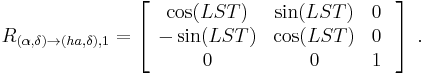
\includegraphics[scale=0.6]{Rmatrix.png}
\caption{an example of a matrix that changes an array of one coordinate
  system to another}
\label{Rmatrix}
\end{figure} 
For this lab, there were transformation matrices that started with our
location in longitude and latitude, but we needed to correct for the
objects in the sky in azimuth and altitude. 

\subsection*{Use of Scripts}
Data for this lab was taken using Kevin Yu's script.

\section*{Results}
A majority of these these data sets were taken horizon to horizon, and
resulted in varying results, from very good data for the Crab Nebula and
the Sun to questionable data for moon measurements. 

\section*{The Crab Nebula}
\subsection*{Declination}
To determine the declination angle of the crab nebula we needed to fit
our smoothed crab nebula data (to reduce the effect of the DC offset of the data) with the equation
\begin{equation}
  F(h_{s}) =
  Acos[2\pi(\frac{B}{\lambda}cos(\delta))sin(h_{s})]-Bsin[2\pi(\frac{B}{\lambda}cos(\delta))sin(h_{s})]
\end{equation}
where we treat A and B as unknown and as the things we want to solve for
using the least
squares method. \par
The smoothing involved using the 'boxcar' method of averaging, where
within an arbitrarily sized box, the median of two peaks would be
created as a data point and then the procedure would move on to the next set of points eventually creating a
trace of the original data with a smoother curve. This is meant to
reduce the homing of the telescopes made during
observation, as well as other anomalies that could have tampered with the
data; unnecessary noise. \par
What we know is that this point source is at a fixed right ascension so
for the data going into $h_{s}$ we must subtract it's known right
ascension from the local sidereal time (lst) data and convert to radians. We also assume that
we know B, c, v and by extension l ($\lambda$ in the equation), which are 10 meters for the baseline,
the speed of light, 10.67 GHz and $\frac{c}{v}$ respectively. The most
important part of this is to create a 'guess' for the value
$sin(\delta)$ by picking values for q between 19 and 24 degrees and
using least squares to  generate a graph of $\chi^2$ versus the guessed
angle.\par
After running this code we got a value of about 22.34 degrees which
was very close to the true declination of the crab nebula, 22
degrees, as seen by the following graph.
\begin{figure}[H]
\centering
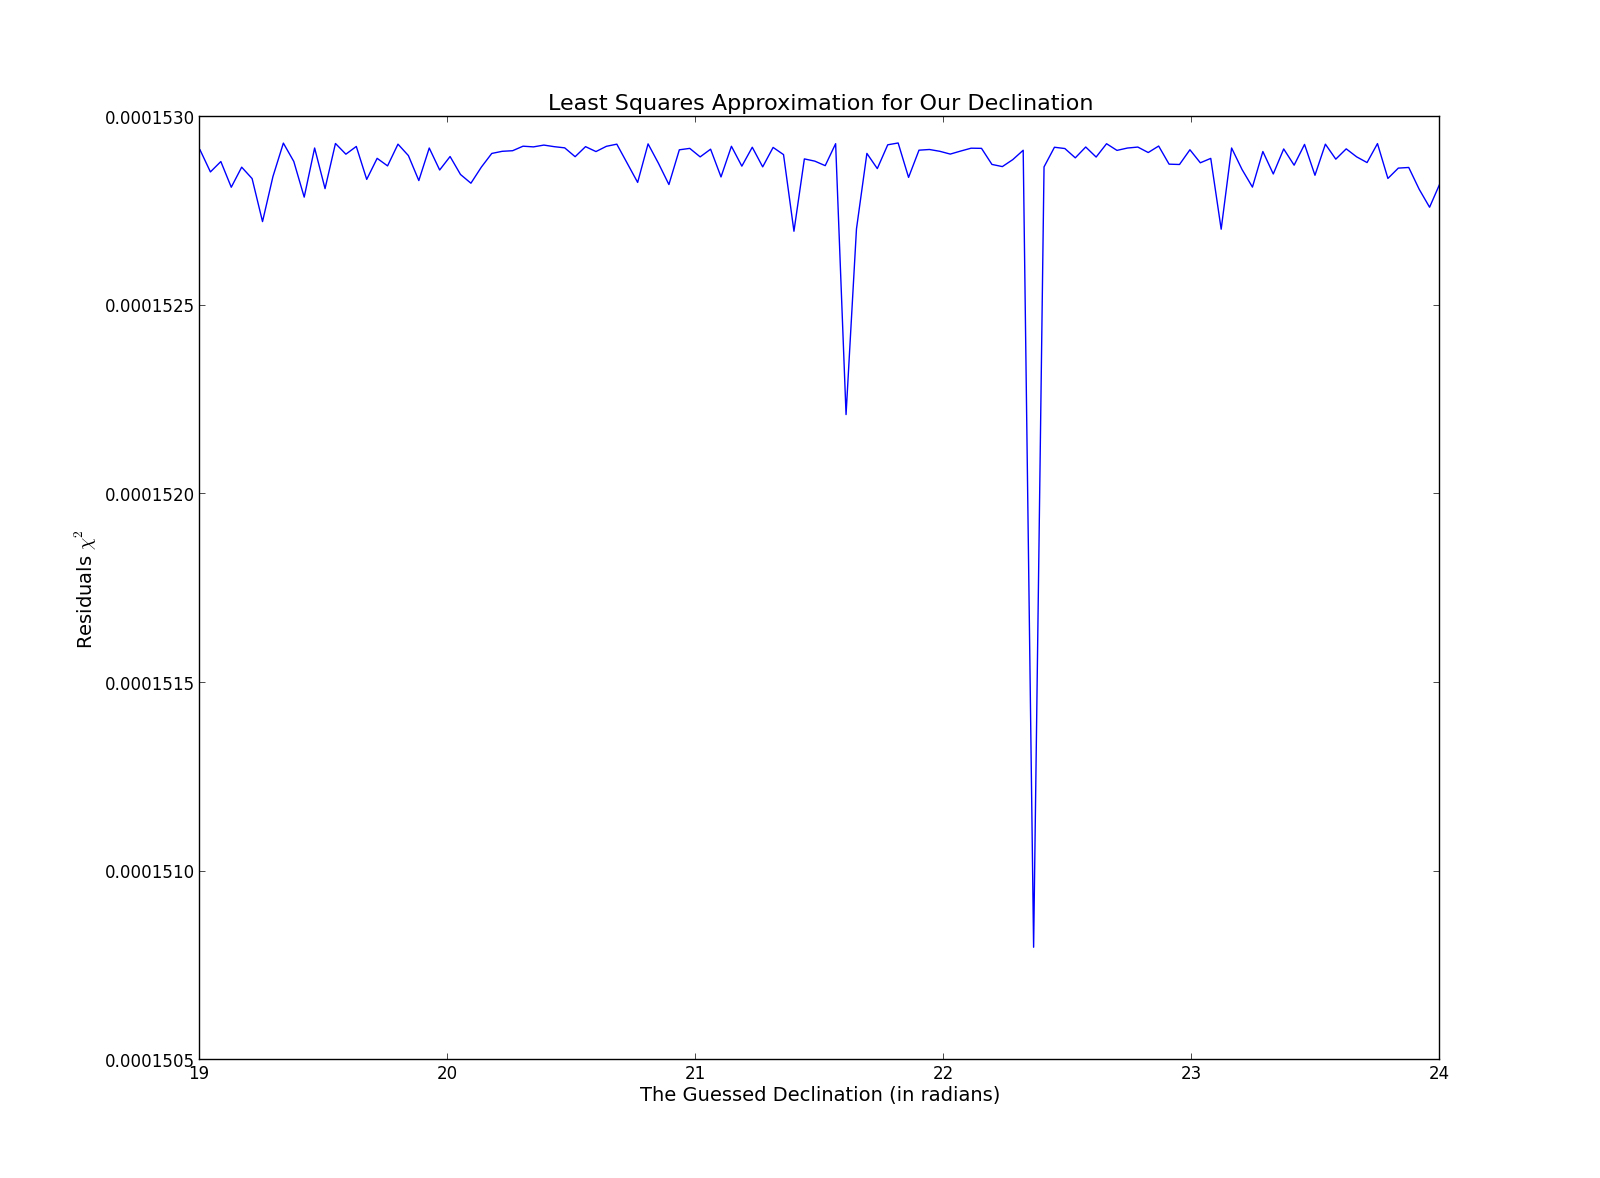
\includegraphics[scale=0.45]{crabdec.png}
\caption{A graph of $\chi^2$ versus declination in degrees for the crab nebula, the
  importance of $\chi$ is that it represents an error that when squared, the closer it is to 0, the more certain we can be that the
  value at minimum $\chi^2$ is the correct one to a higher degree of confidence, and the model agrees
  closely to the true declination}
\label{crabdec}
\end{figure} 
We see a sharp decrease in $\chi^2$ near where the observed declination
angle should be, and there are no other points nearly as steep as the one
at about 22.3 degrees, which closely agrees with the true declination
angle of 22 degrees; a calculation within a percent of the observed
value.
\subsection*{Cable Length}
From the code, The matrix a could be called which housed the values of A
and B  which are equal to $cos(2\pi*v\tau)$ and $sin(2\pi*v\tau)$
respectively. For both, we get a value of the order $10^-6$ which after
plugging in and solving for $\tau$ and multiplying that by the speed of
light,  we get a value of about .007 meters,  which comes out to about a
1 cm cable difference length. 
\subsection*{Baseline}
As a way to make sure that the previous method of least squares is
correct(a failsafe), the code was modified so that $\delta$ could now be assumed to
be what is in the lab packet, and instead make guesses for B, the
baseline. Again the data for the crab nebula was smoothed out via the
boxcar method again, and much of the code was left alone except now the
declination was assumed instead of the baseline. Now the 'guesses'
made ran between 7 meters and 12 meters, with a guess being made every
.05 meters. After going through all the guesses, the code came out with
a best guess of 10.027 meters, which is less than a percent within the
actual (assumed) value of 10 meters. Below is the graph for this run.
\begin{figure}[H]
\centering
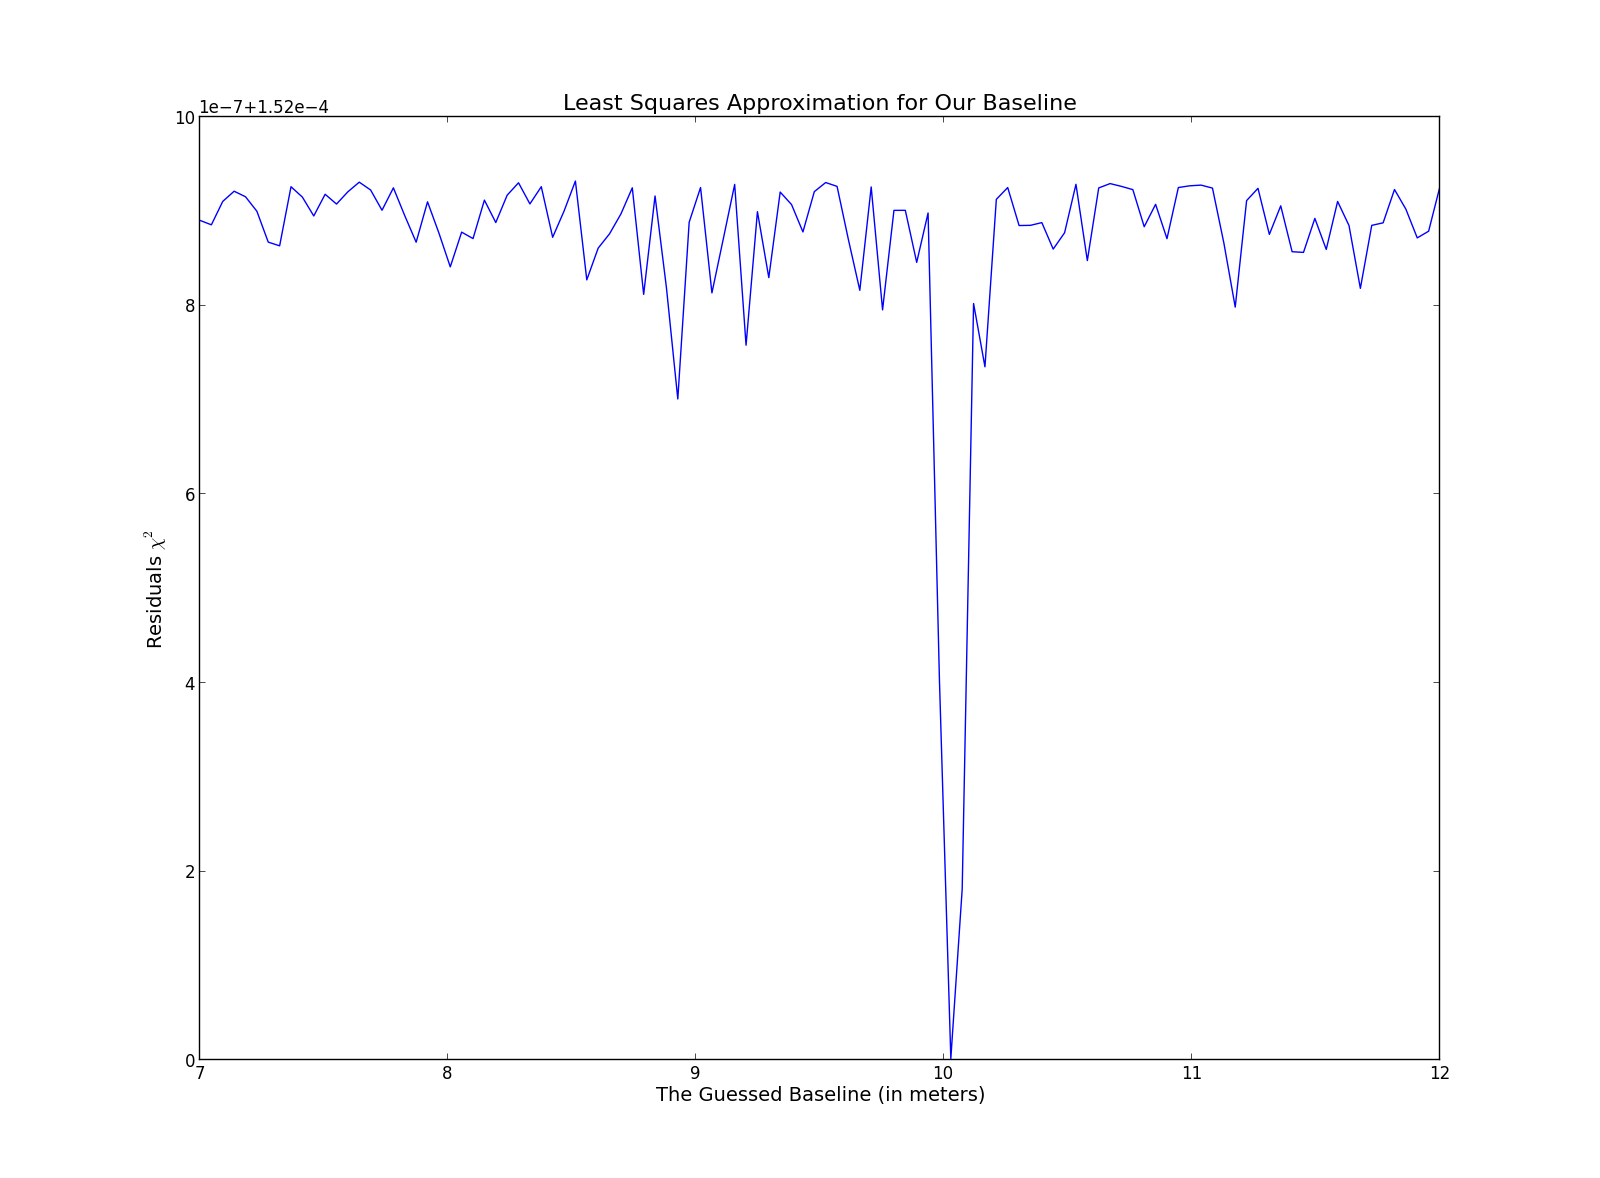
\includegraphics[scale=0.45]{crabbaseline.png}
\caption{A graph of $\chi^2$ versus the guessed baseline length in
  meters, again there is a single large dip to near zero for $\chi^2$
  meaning that the value of 10.027 meters was the best fit for this data}
\label{crabbaseline}
\end{figure}
This baseline data together with the declination data indicates that the
data gotten from the telescope is accurate(after smoothing), because our code was
accurately written to track this source.\par
\subsection*{Previous Attempts and their Solution}
 On previous attempts, nearly all of the data was not viable for data
 analysis because the code was at the time set to chage position to
 continue tracking the object every 2 minutes. Because of this, our
 sources easily got out of range within a few hours, resulting in a lot
 of noise in our data. Our tracking beam
 was not concentrated on the source but would be instead on tangent
 to the source after a while, losing power that the telescope would have
 collected. With an update to track every thirty seconds made, the data came
 out better than before. 
\subsection*{Least Squares Fit}
Using the same code to guess a baseline, a graph was generated plotting
the smoothened data set with YBAR, the best fit line for the data
set, our observing time was relatively short so the whole set rather
than a window was fitted. Below is the result
 
\begin{figure}[H]
\centering
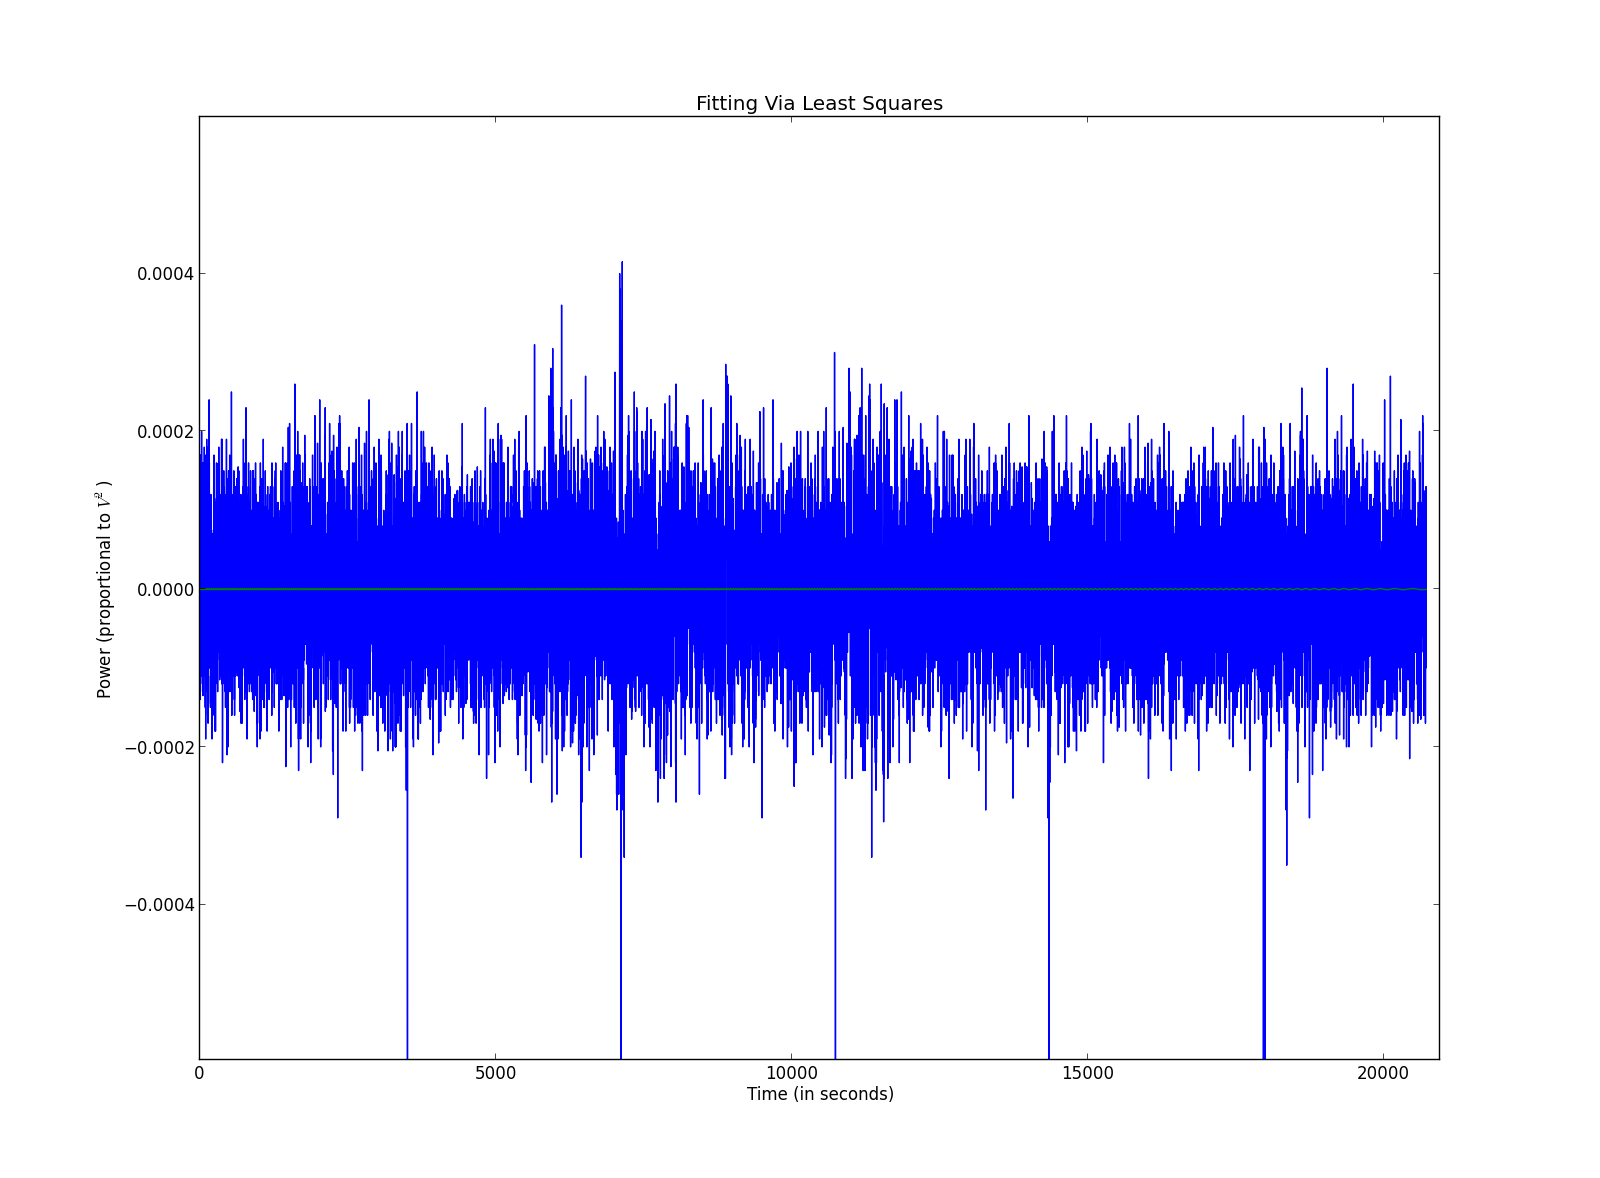
\includegraphics[scale=0.45]{crablsqfit.png}
\caption{The least squares fit for the smoothened crab nebula data,
  from this vantage point, the best fit line can only barely be seen}
\label{crablsqfit}
\end{figure}

We do not see much from here, the least square fit line seems to emulate
a straight line since the data set doesn't seem to have a sinusoidal form, it's
more like a straight line. The reason it could look like this is because it
is so far away that the Power Spectrum appears to be constant, especially
over a relatively short time interval (we did not take a whole horizon
to horizon observation). Now, if we were to zoom in  on the best fit line 

\begin{figure}[H]
\centering
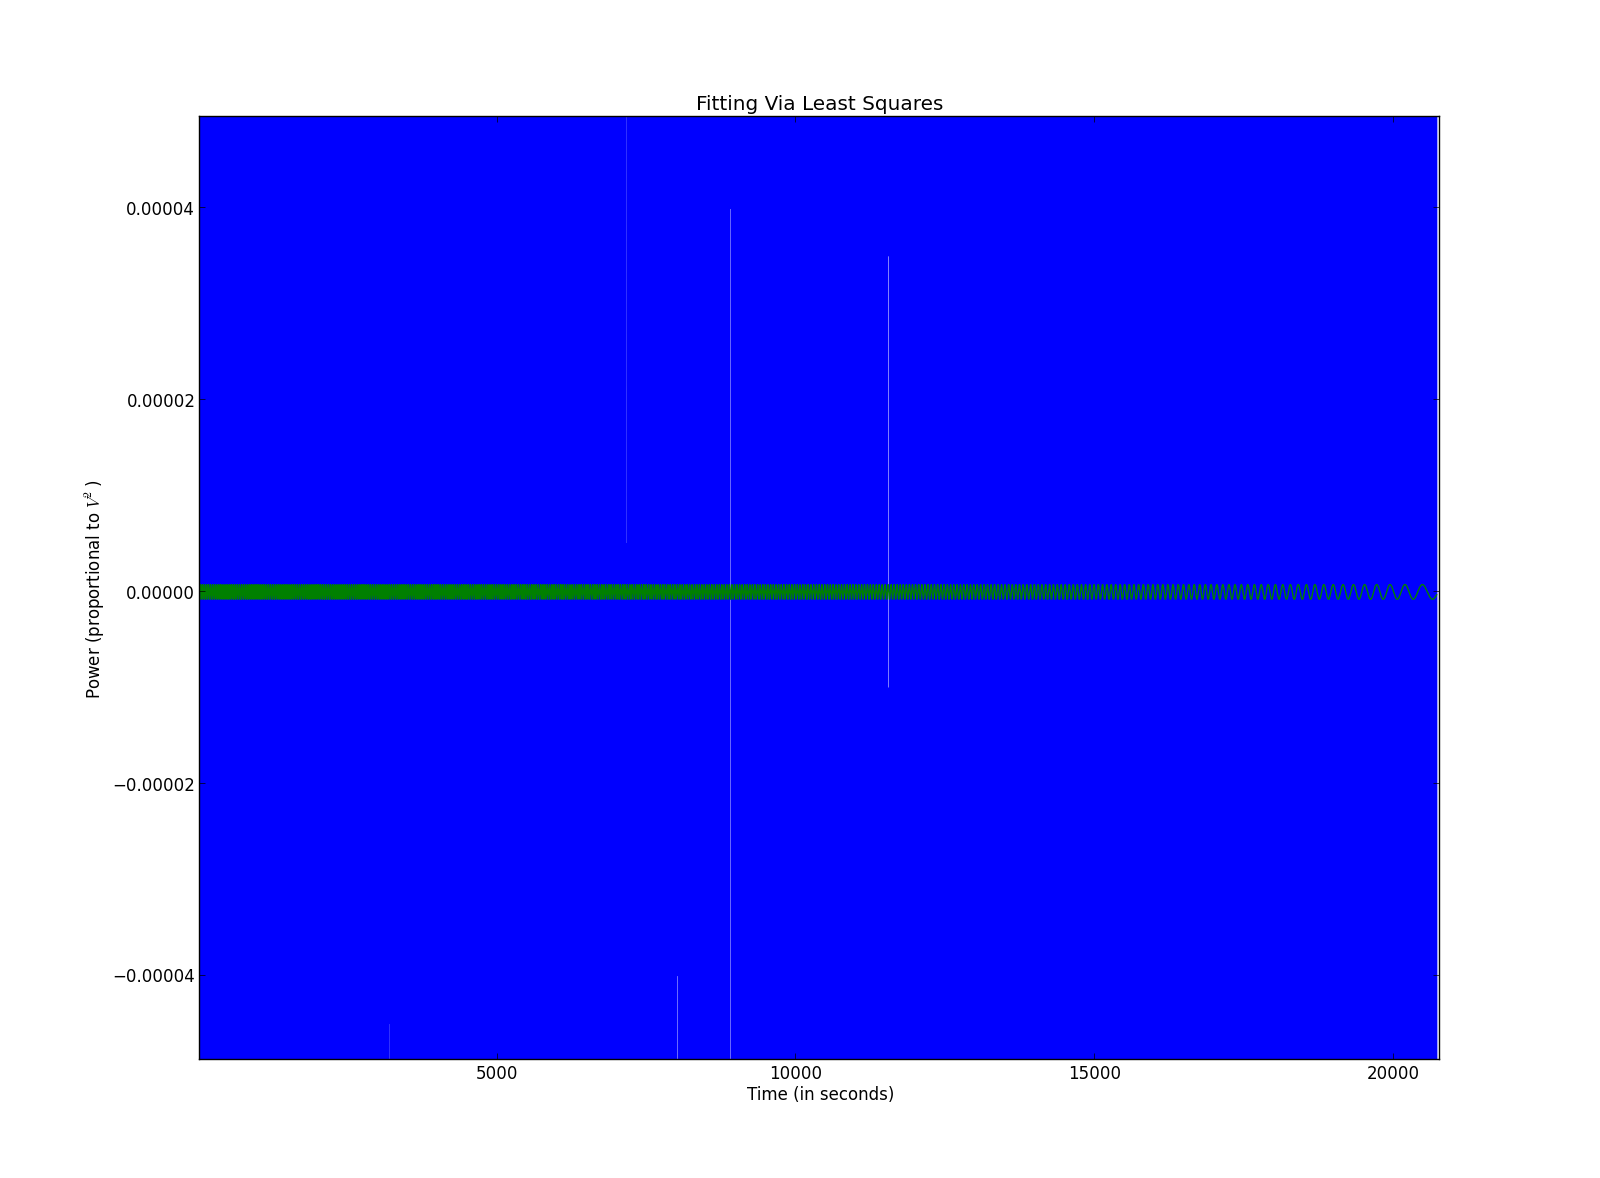
\includegraphics[scale=0.45]{crablsqfitzoom.png}
\caption{The same graph as before but where we zoom in on the best fit line}
\label{crablsqfitzoom}
\end{figure}

In this zoomed in picture, we see that the best fit line is a sine wave
whose wavelength increases as time passes. This can be explained by the
time when we chose to observe it. We started observations when the
Nebula was already at its peak and so the signal was at its strongest,
and as it neared and passed the horizon, it's
wavelength was lengthened and the signal gradually became weaker.  
\section*{The Sun}
We observed the Sun again after updating our tracking time for the majority of the day, missing out on
the first hour or so of data.
\subsection*{Phi}
With the sun data, it was important to choose an area of the data that
resembles a parabola so that the appropriate value of $\phi$ could be
chosen and so that a envelope could determine how well our choice of
$\phi$ was. For this sun data, the window of data points 1700 to 3300
(we took one data point per second) contained an
area that had a parabolic shape so between these points. With this, we
begin to find a
$\phi$ according to the fitting equation

\begin{equation}
F(t) = cos((B/l)cos(\delta)cos(hour_{angle} + \phi))
\end{equation}
 
for which we have to minimize for $\phi$. The hour angle is not
like the point source, it is always changing since the Sun is an
extended point source so it had to be adjusted by
subtracting the right ascension array from the lst array to give us an
hour-angle array, which then has to be converted to radians. In addition,
as mentioned, there was focus on a parabolic area of the Sun
Data. Another detail that had to be dealt with was the DC offset of our
data, to deal with this, the mean value of the 'volts' data was
subtracted off of the original 'volts' data, this is not the most
effective way to account for DC offset but for fitting purposes it is acceptable. After making sure to have
all arrays match in dimension; all arrays must cover the same
place with the same lengths, we made a guess in $\phi$ and we see that
from the graph, we get a $\phi$ value of 2.06266 radians.

\begin{figure}[H]
\centering
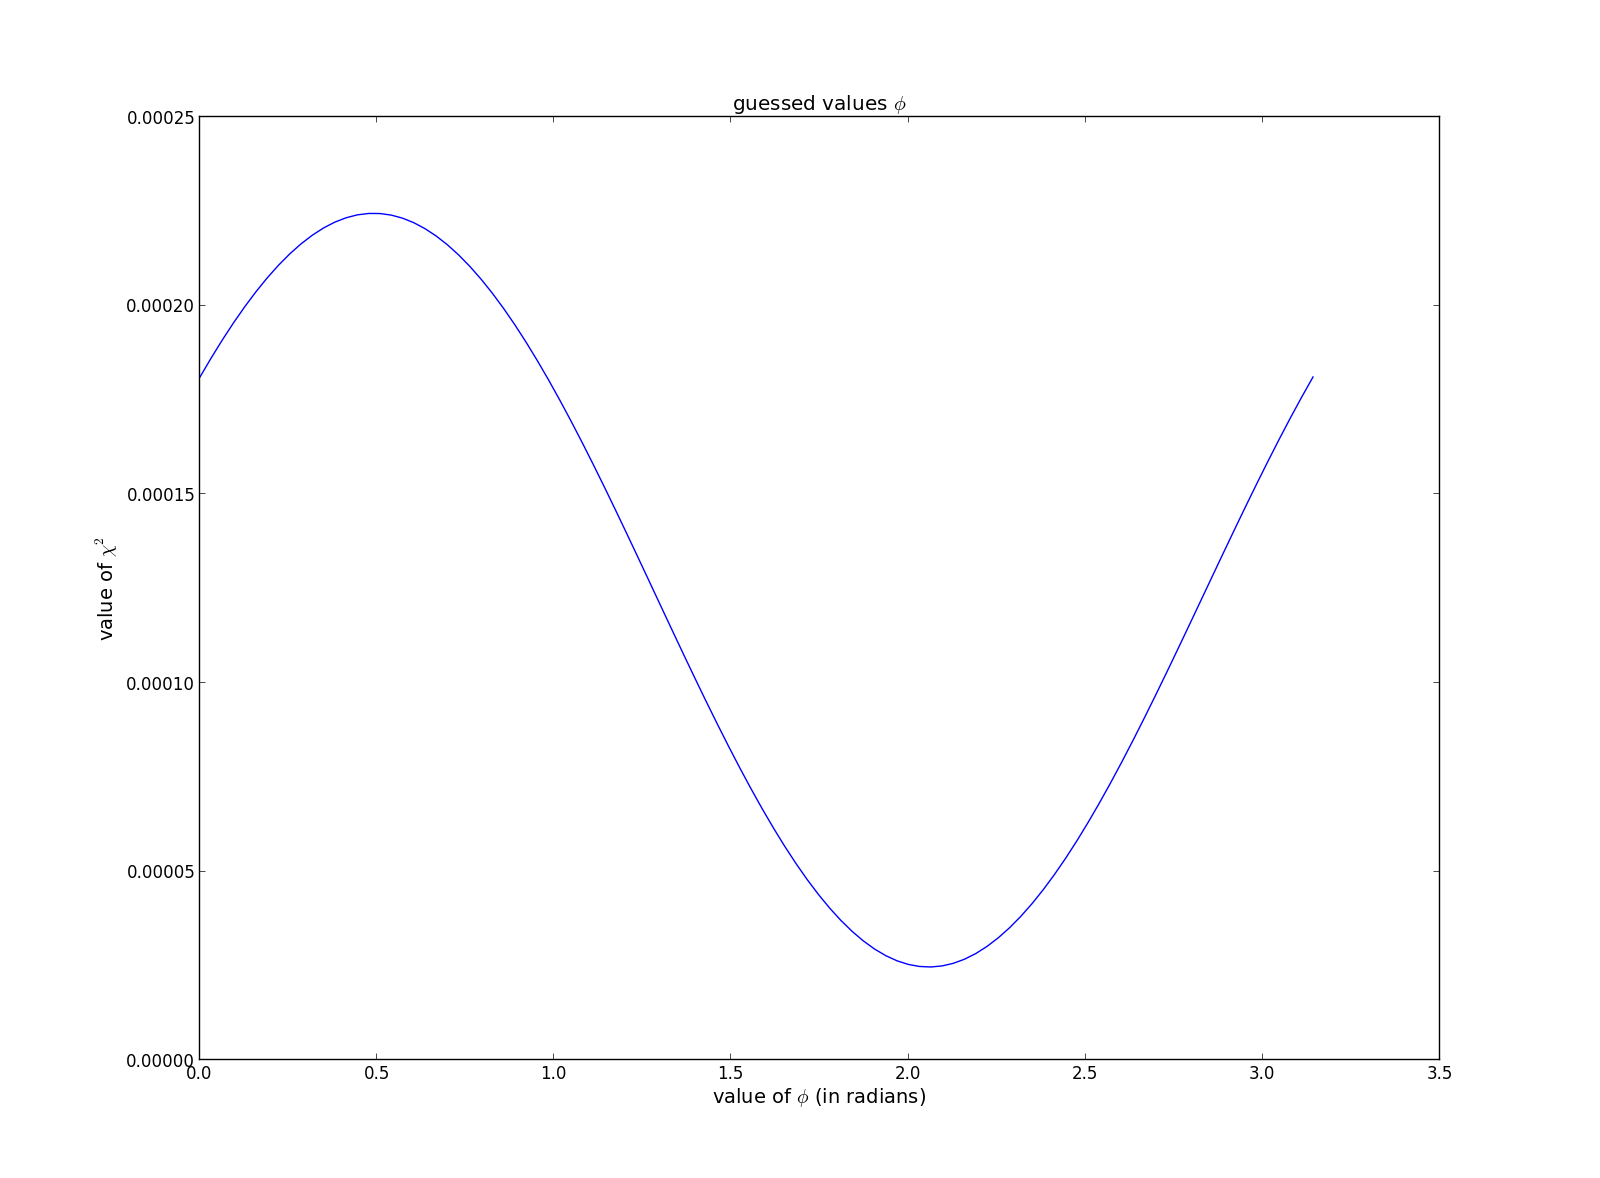
\includegraphics[scale=0.45]{sunphi.png}
\caption{A graph of $\chi^2$ versus guesses in $\phi$, we see a strong
  peak towards zero at the value of about2.062.}
\label{sunphi}
\end{figure}
 
As we see, the graph looks like a sine wave, the reason perhaps being that
for $\phi$ this trend is periodic since it the $\phi$ is in a cosine function, and
since it's in radians, its behavior must be periodic. 
\subsection*{Least Squares Fitting}
To fit a least squares fit to our data at the parabolic area, all we do
is plot our Y array which is defined as the volts data of the sun minus
the mean of that same data, again to compenstae for the DC offset. And
plot that against the YBAR dta, which is the best fit line for the data acquired,
plotting these, we get,   
\begin{figure}[H]
\centering
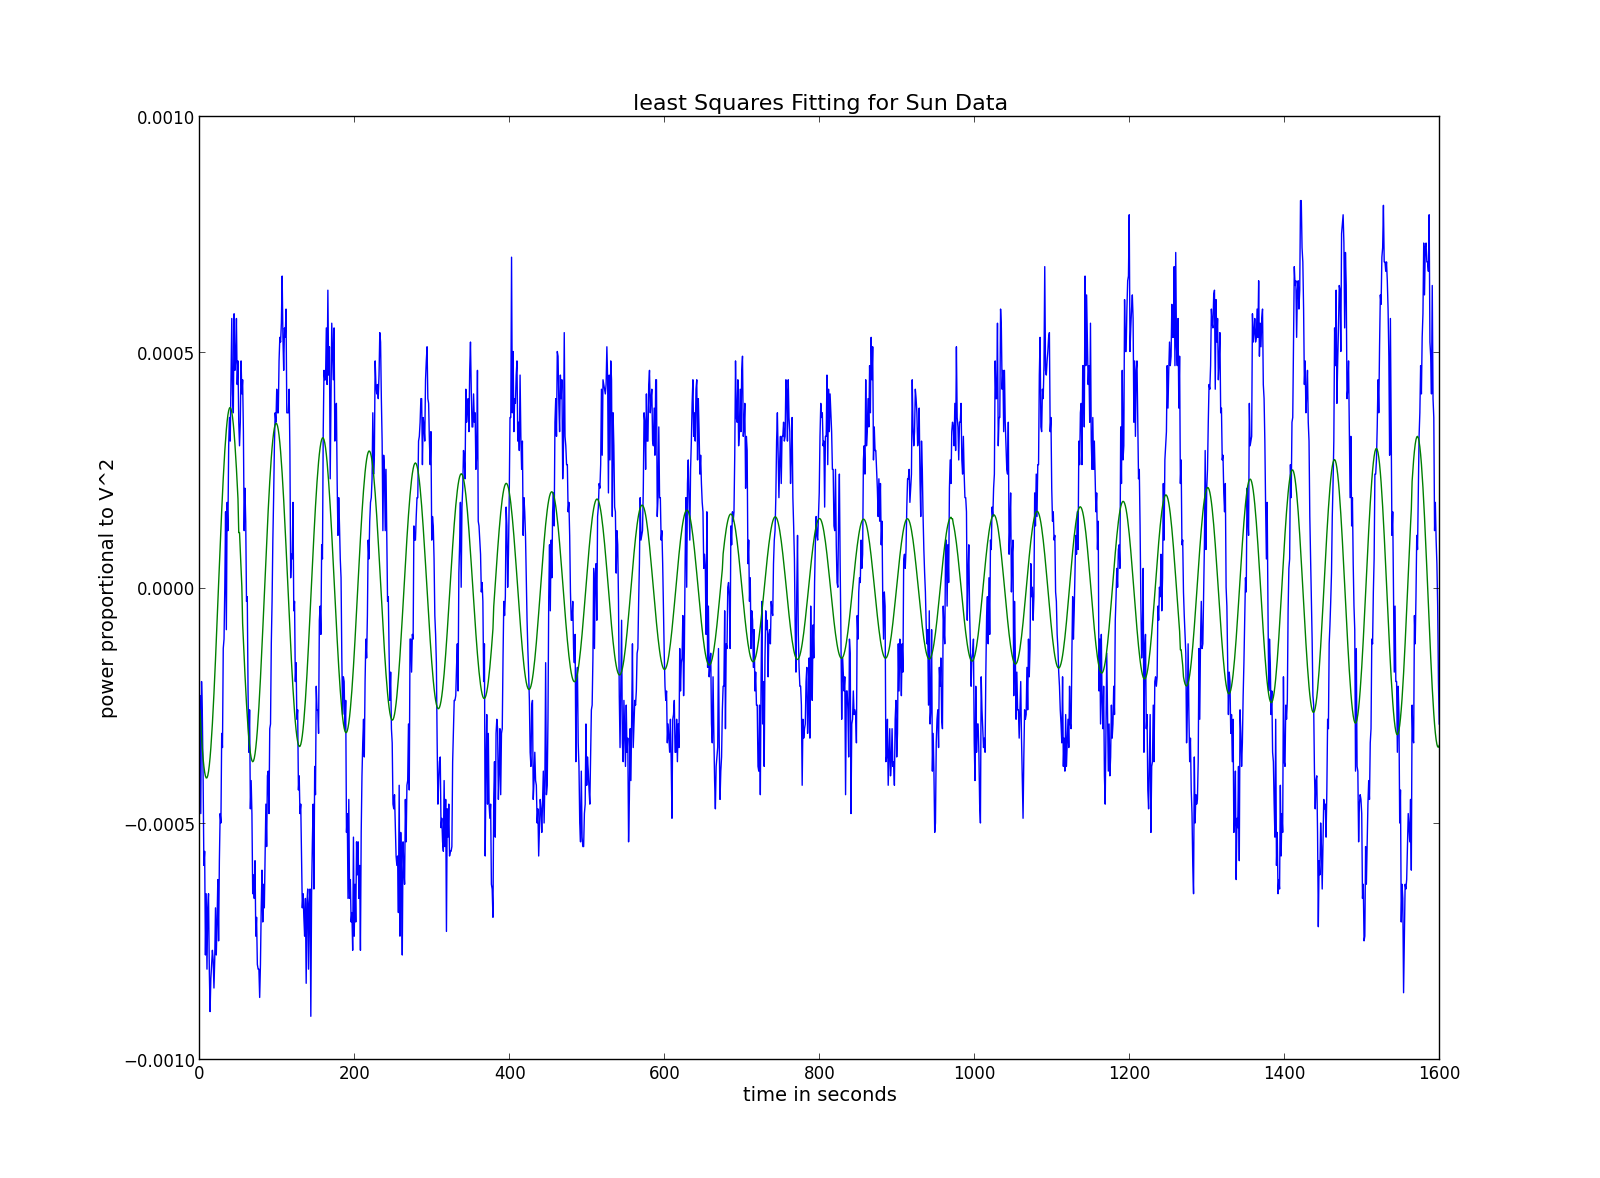
\includegraphics[scale=0.45]{sunlsqfit.png}
\caption{Fitting for our Sun Data, the best fit data fits well with the
  sun data.}
\label{sunlsqfit}
\end{figure}
This least squares fit line does an excellent job in approximating the
wavefront of this window of values,  so that a pattern can be seen more easily.
\subsection*{Envelope}
To fit for an envelope around our data, that is where our minimized
$\phi$ comes in when plugging it into our modulation function
F(t). After plugging this value into our equation, we can plot YBAR as
well as a negative version of it too, after doing both of these our
result is
 
\begin{figure}[H]
\centering
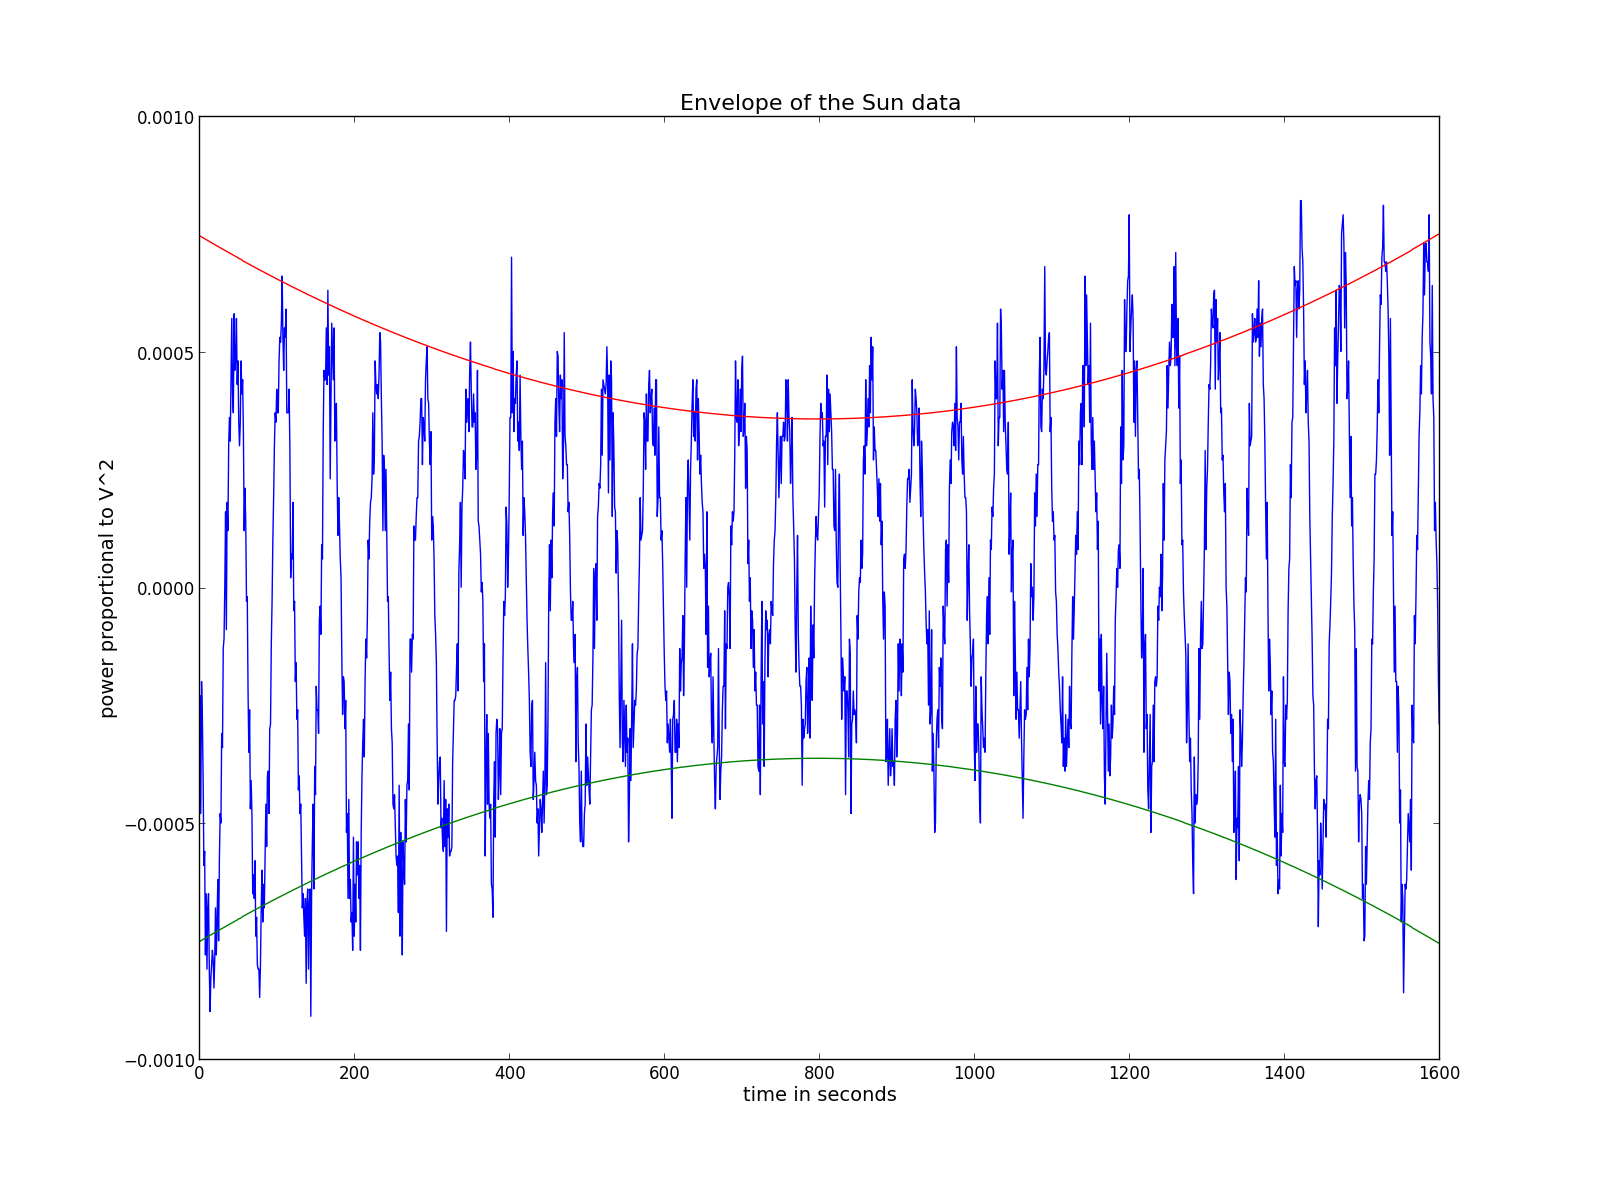
\includegraphics[scale=0.45]{sunenvelope.png}
\caption{A good approximation of the envelope encasing the data set to a
good degree, the envelope correctly approximates and averages
over the peaks of the individual spikes to create a single wave
describing the data.}
\label{sunenvelope}
\end{figure}
This enveloping line is the result of graphing YBAR with the Sun data,
the importance of YBAR becomes apparent when trying to measure the
radius of the sun. 
\subsection*{The Radius of the Sun}
To find the radius of the sun, it is necessary to plot the $MF_{theory}$
versus the product of fringe frequency and R; fR. A combination that
minimizes MF has to be a zero cross section and so we can use that to
find an R, by looking at our YBAR array's minimum value and using
indexes to find the concurrent values of declinations, right ascensions,
lst's and using those values to find a value of $f_f$,  known as the
fringe frequency. With this fringe frequency we can find the value of R
by dividing the value crossing zero on a bessel function by the fringe
frequency to get R,  the radius of the Sun. Shown below is the bessel
function for the Sun. 
\begin{figure}[H]
\centering
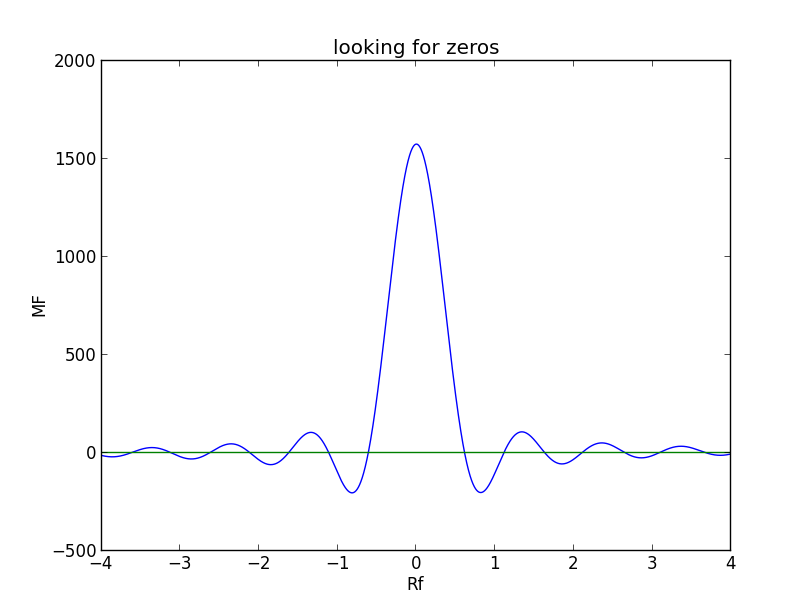
\includegraphics[scale=0.5]{zerosR.png}
\caption{The Bessel Function for the Sun}
\label{zerosR}
\end{figure}
 Another detail in the parabolas we try to find is
their cause. When the dishes point toward the sun, some of the
waves-fronts may experience destructive interference, which we see on
the graphs as parabolas or dips. These are actually related to the
fringe frequency. There can be different values of R in the combination
fR but when at a local minimum \ref{zerosR} we can get the lowest
values of the angles needed in the fringe frequency so that we can just
divide the value at which the x-axis crosses 0 by the fringe fraction
to get the Radius of the Sun in radians \par
The only unfortunate part that while calculating R, we came across a
value of .025 radians which is a factor of 10 larger than the true
radian radius of the Sun. Attempts to fix this radius measurement
wielded nothing since choosing a larger R only madethe radius larger
than it already should be. The error could have been in the code run to
get the values for $\delta$ and $h_{s}$, or more likely, human error
while attempting to compute the radius by hand. 
\subsection*{The Moon}
This data is treated identically to the sun data save for some
modifications and regions of interest. Unfortunately this data did not
yield any good data to use least squares on, so the data presented
here may not be favorable.

\subsection*{Phi}
Again, using the same procedure that was used on the sun,  get a $\phi$
of 2.79 radians,  since data was taken from an area that had a
'half-parabola' shape so this $\phi$ may not be all that reliable. A
note should be made that the moon data was smoothened out, so this data
is not useless since the DC offset has been at least partially dealt
with. 
\begin{figure}[H]
\centering
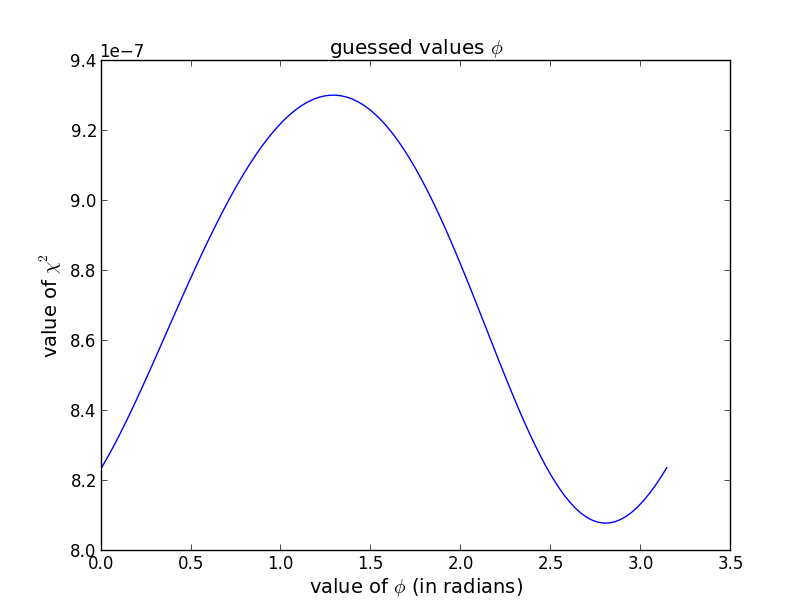
\includegraphics[scale=0.5]{moonphi.png}
\caption{A graph of the the most favorable guess for $\phi$ based on the
value of $\chi^2$}
\label{moonphi}
\end{figure}
\subsection*{Least Squares Fitting}
Using this value of $\phi$, we again calculted the array for the best
fit line of our data interval  and resulted in 
\begin{figure}[H]
\centering
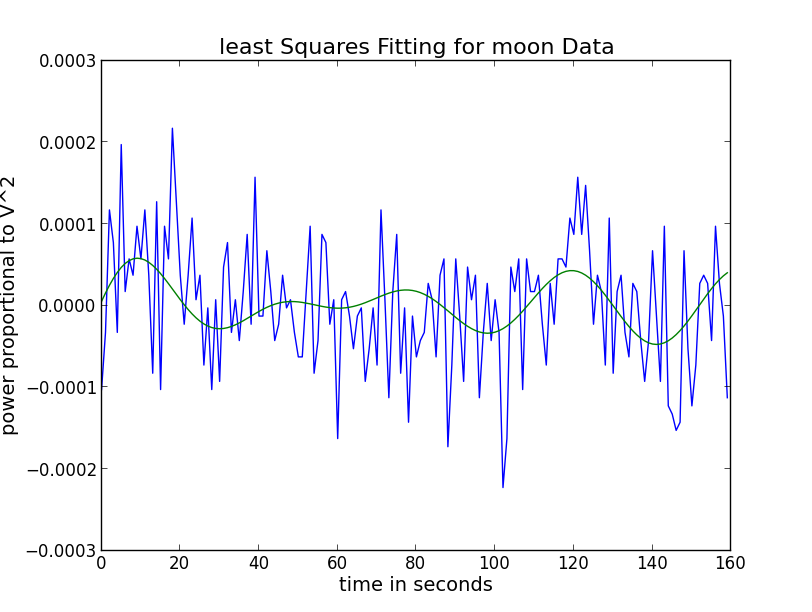
\includegraphics[scale=0.5]{moonlsqfit.png}
\caption{The least square fit line for the data on some interval of the
  whole set}
\label{moonlsqfit}
\end{figure}
we see that the least squares fit line does accurately fit the data, so
perhaps the $\phi$ from the previous section is more accurate than
previously thought.
\subsection*{Envelope}
As for the envelope, when it is overliad over the smoothed data, it
does not look right, mostly because the enevelope does not go over the
peaks of the data points, the data range selected is not parabolic. 
\begin{figure}[H]
\centering
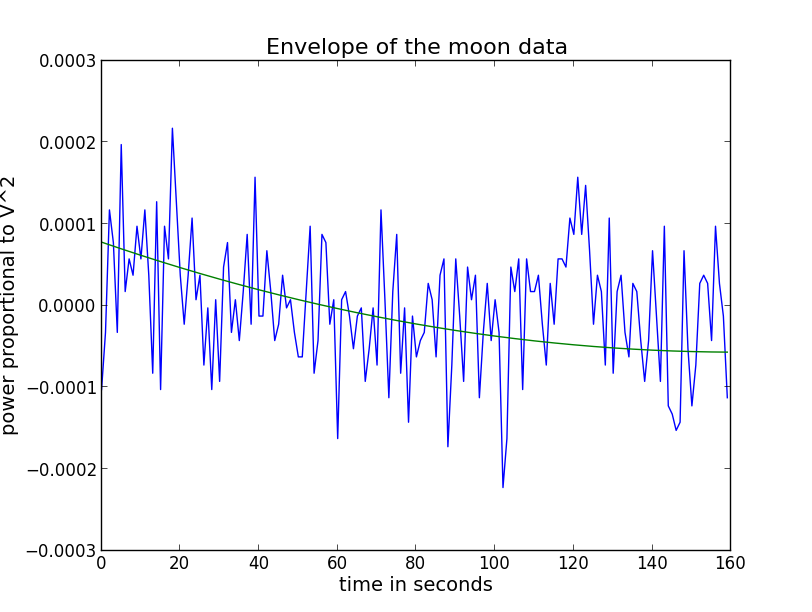
\includegraphics[scale=0.5]{moonenvelope.png}
\caption{The supposed envelope of the moon data, it is wrong mostly
  because of the bad data}
\label{moonenvelope}
\end{figure}
Since we did not choose a window with a minimum, $\phi$ could not be
accurately measured, so that will affect the radius measured.

\subsection*{Radius}
Once again we would have some minimumparabola to look at,  but from the
moon data gathered there did not seem to be any good areas to pick a
minima. 

\section*{Conclusion/Discussion}
Overall, the results were satisfactory, being able to get a measurement
that worked with least squares approximations with two different
sources did at least affirm that tracking codes were working. The
problem was mainly with the moon data that did not seem to be good data
to work with, which may be because it wasn't reflecting fully as it was
in previous weeks. Even after smoothing the moon data,  it still weilded
bad results for the envelope because of its irregular form over larger
windows. Though there was the start of being able to calculate the
Radius of the Sun, it could not be finished due to a lack of
understanding the locations of the minimum values in the arrays, Radii
couldn't be fully completed. 


\end{document}